\documentclass[journal=jpcafh,manuscript=article,layout=onecolumn, 12pt]{achemso}
\usepackage[version=3]{mhchem} % Formula subscripts using \ce{}
\usepackage[T1]{fontenc}       % Use modern font encodings
\usepackage{amsmath}
\usepackage[dvipsnames]{xcolor}
% NB added command for in line cite
\newcommand{\onlinecite}[1]{\hspace{-1 ex} \nocite{#1}\citenum{#1}} 
%
\author{Benjamin~A.~Laws}
\affiliation{School of Chemistry, University of New South Wales, Sydney NSW 2052, Australia}
\author{Olha Krechkivska}
\affiliation{School of Chemistry, University of New South Wales, Sydney NSW 2052, Australia}
\author{Callan M. Wilcox}
\affiliation{School of Chemistry, University of New South Wales, Sydney NSW 2052, Australia}
\author{Klaas Nauta}
\affiliation{School of Chemistry, University of New South Wales, Sydney NSW 2052, Australia}
\author{Scott H. Kable}
\affiliation{School of Chemistry, University of New South Wales, Sydney NSW 2052, Australia}
\author{Timothy~W.~Schmidt} 
\email{timothy.schmidt@unsw.edu.au}
\affiliation{School of Chemistry, University of New South Wales, Sydney NSW 2052, Australia}
\alsoaffiliation{ARC Centre of Excellence in Exciton Science, Australia}
\title{Intramolecular Hole$-$Transfer in Protonated Anthracene}
\abbreviations{PES,PAD,EA,eKE,FWHM,VMI}
\begin{document} 
\begin{abstract} 

Excitation spectra of protonated and deuterated anthracene are obtained by triple-resonance dissociation spectroscopy. Very cold cations, protonated/deuterated exclusively at the 9-position, are generated from two-colour two-photon threshold ionisation of 9-dihydroanthracenyl radicals. The excitation spectra reveal rich structure, not resolved in previous studies, that is assigned based on full anharmonic and Herzberg-Teller coupling calculations. This work confirms that excitation of protonated anthracene induces a symmetry-breaking intramolecular charge-transfer process, where the positively charged hole hops from the central bridging sp$^2$ carbon, onto one of the aromatic rings. Signatures of this charge-transfer event are observed in the excitation spectrum, through active Herzberg-Teller progressions.

\end{abstract}
\section{Introduction}
Charge transfer between two different molecules in an excited electronic state is at the heart of photosynthesis~\cite{wah14}. This process is also mimicked in artificial devices which generate solar energy. In both organic photovoltaics (OPV) and dye-sensitized solar cells, following photon absorption, the excited state migrates and undergoes a charge transfer event~\cite{cor19,zhe17,lis11}. A detailed understanding of charge separation in OPV is hampered, in part, by the impossibility of detailed quantum chemical calculations on such a large system. In OPV devices, the electrons and holes are then conducted to metallic electrodes through a series of inter and intramolecular electron and hole-transfer processes.

Gas-phase laser spectroscopy offers the possibility to interrogate a well-defined, cold, isolated chemical system which is tractable at quantitative levels of electronic structure theory. To study photo-induced hole-transfer, a charged species must be studied, which engenders further experimental difficulties. Cations can be introduced into the gas phase by electrospray ionization, but the resulting species are not cold~\cite{pal21,kno09,lor07,nob15}. Jet-cooled molecules can be ionized in the expansion region, but unless the ionization is at threshold, requiring tunable vacuum ultraviolet radiation, excess energy can be deposited in the cation~\cite{ala10,cha09,ala10b,ala13,kre13}. Techniques capable of studying jet-cooled, isomer-selected, cold cations are thus desirable.

The C$_{60}^+$ cation was recently studied by the photodissociation of its adduct with helium atoms in a 22-pole cryogenic ion trap. This technique affords a spectrum with a very small shift from the true gas phase spectrum. For C$_{60}^+$ cation this was sufficiently small to confirm the present of C$_{60}^+$ in interstellar space~\cite{cam15}. Recently, we reported a triple-resonance technique whereby nascent cations were resonantly photodissociated following preparation by a resonant two-colour two-photon photon ionization process, at threshold. The result was an unambiguous spectrum of protonated naphthalene, isomer selected and vibrationally cold~\cite{kre13}. Here we extend this treatment to protonated anthracene, which demonstrates symmetry-breaking in the excited state along a Marcus-Hush-like charge transfer coordinate.

%Protonated polyaromatic cations PAH+ are also of considerable interest to astrochemistry, as their abundance in the interstellar medium (ISM) makes them promising candidates for diffuse interstellar band (DIB) carriers~\cite{mey21}. %While early photostability studies suggested that only relatively large (>50 C atoms) PAH molecules could survive in the ISM~\cite{joc94}, more recent studies have shown that structure also plays an important role. A Photoionization Mass Spectrometry experiment of a variety of PAHs showed that the Anthracene structure was relatively photostable, and is predicted to survive in regions of the ISM~\cite{joc99}. Despite this interest in



Protonated anthracene has been studied previously, as its relatively high photostability~\cite{joc99} and abundance in the interstellar medium (ISM) suggest it is a promising candidate to be a diffuse interstellar band (DIB) carrier~\cite{mey21,tie08,hud01,pat08}. However, previous reports are neither at rigorously low vibrational temperature, nor isomer-selected. Alata \emph{et al.} measured the photo-fragmentation spectra of protonated anthracene, which was created (along with other PAHs) in an electrical discharge containing H$_2$~\cite{ala10}. Through comparison to RI-MP2 calculations, structure observed around 491~nm was assigned to the $\text{S}_1\leftarrow \text{S}_0$ transition of the 9H-An$^+$ isomer. A subsequent absorption measurement of protonated anthracene held in a cryogenic matrix by Garkusha~\emph{et al.} exhibited several spectral bands across the 400-500nm region~\cite{gar11}. They instead assigned the structure around 491~nm to the $\text{S}_2\leftarrow \text{S}_0$ transition of the 1H-An$^+$ isomer, based on TD-DFT B3LYP calculations. A recent computational study has suggested the initial assignment to the 9H-An$^+$ isomer was correct, however this discrepancy highlights the need for experimental isomer selectivity~\cite{li21}. More recently, electronic spectra of protonated anthracene have been measured via helium-tagging action spectroscopy, however this technique is also limited by isomer non-selectivity and spectral resolution~\cite{mey21}.

In this study, we prepare 9-hydroanthracenium cations exclusively in their vibrational ground state by two-color resonant ionization of the corresponding 9-dihydroanthracenyl radical. Subsequent resonant photodissociation of the cation reveals the isomer-selected $\text{S}_1\leftarrow\text{S}_0$ spectrum of 9-hydroanthracenium. We show that the $C_{2v}$ ground state undergoes symmetry breaking in the excited state along a $b_2$ (in-plane) mode, effectively localizing the positive charge on one end of the molecule. This coordinate thus represents the abscissa of a Marcus diagram, and the excitation spectrum is interpreted from this standpoint.

\section{Theoretical Considerations}
Anthracene protonated at the 9-position is considered $C_{2v}$ until proven otherwise. If the sp$^3$ carbon is considered as an insulator, the chromophore will consist of two aromatic rings linked by an sp$^2$-hybridized bridging carbon. The frontier orbitals of the aromatic rings can be taken in even and off combinations, resulting in sets of $b_1$ and $a_2$ symmetry. Only the $b_1$ set can interact with the bridge, which is also $b_1$. Of the highest occupied aromatic $b_1$ orbitals, one will have a node at the tertiary carbon atom adjacent to the bridge, and is not expected to be strongly perturbed. The other mixes with the bridging p-orbital and is lowered in energy. This results in two relatively unperturbed aromatic, symmetry-adapted orbitals of $a_2$ and $b_1$ symmetry. The lowest-energy unoccupied orbital is largely located on the bridge. The frontier orbitals are shown in Figure~\ref{Fig:1}.

\begin{figure} [h]
	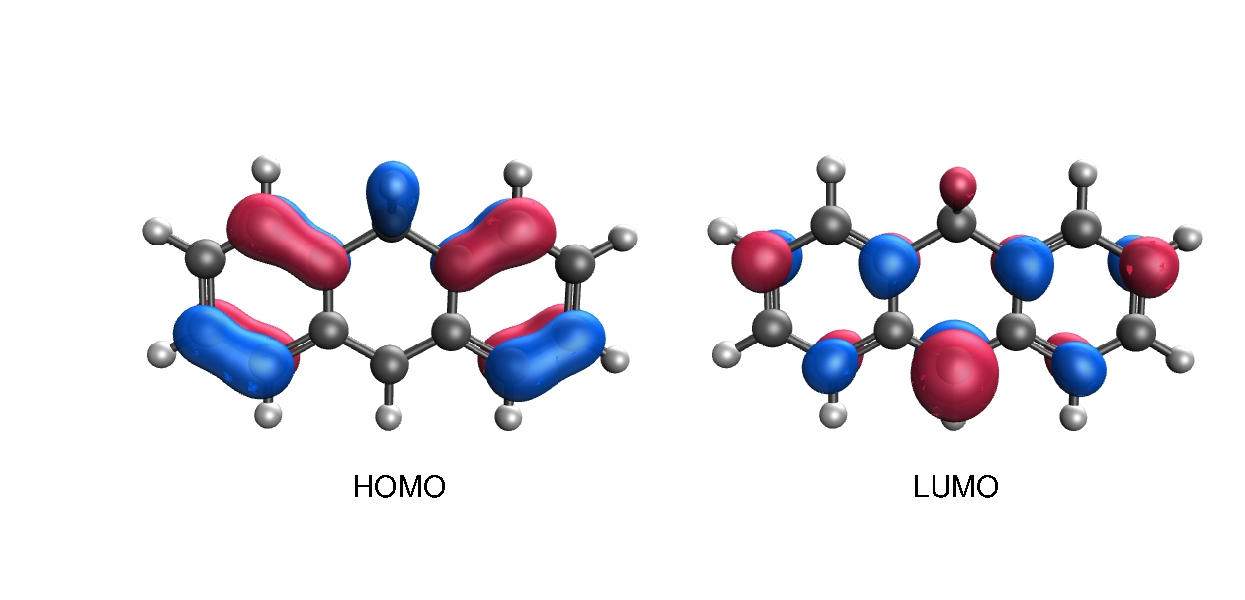
\includegraphics[width=0.8\textwidth]{figures/Figure1}
	\caption{Frontier orbitals of 9H-An$^+$ calculated at the M06-2X/cc-pvtz level. The HOMO has a node at the tertiary carbon adjacent to the sp$^2$ bridge, with electron density largely localised on the aromatic rings. Conversely, the LUMO is largely located on the bridging carbon. Therefore, the HOMO-LUMO transition represents electron transfer from the aromatic rings to the bridge.}
	\label{Fig:1}
\end{figure}

The HOMO-LUMO transition of the cation is thus electron transfer from the aromatic rings to the bridge, corresponding to hole-transfer from the bridge onto the aromatic rings. This brings about two near-degenerate transitions to states of $A_1$ and $B_2$ symmetry. Distortion along a $b_2$ mode will reduce the point group to $C_s$ and render both these excited states $A'$. The interaction between these two states could potentially push the lower state to an energy below that of the $C_{2v}$ geometry.

This description is supported by quantum chemical calculations presented in this work. The ground state geometry was calculated at both the M06-2X/cc-pvtz and CCSD/cc-pvdz levels of theory, with both calculations converging to a planar $C_{2v}$ geometry. All frequencies were found to be real, indicating a true minimum energy. Corresponding TDDFT and EOM-CCSD excited state calculations were also computed for the S$_1$ state, which converged to a planar $C_s$ geometry. This geometry arises from the charge transfer from the bridge onto one of the aromatic rings, causing an in-plane $b_2$ distortion. To interrogate this charge transfer process, a transition state search on the S$_1$ surface was completed using the Berny algorithm of Gaussain16~\cite{g16,ber82}. This search revealed a $C_{2v}$ saddle-point geometry with one imaginary frequency, 35~cm$^{-1}$ above the $C_s$ excited state minima.

The pathway from the $C_{2v}$ to $C_s$ geometry can be described by the intrinsic reaction coordinate (IRC). This was calculated in both the forward and reverse directions using Gaussian16 software and the HPC algorithm, calculating force constants at each step along the path~\cite{hra04}. This revealed a shallow double well potential, as shown in Figure~\ref{Fig:2}(a). The potential energy surface is shown across both the forward and reverse IRC directions, highlighting the $C_{2v}$ saddle point and the two $C_s$ global minima. The coordinate linking the minima through the saddle point represents the abscissa of a Marcus diagram. Potential energy curves of the higher excited $\text{S}_2$ and $\text{S}_3$ electronic states were also calculated along the IRC coordinate, as shown in Figure~\ref{Fig:2}(b). The surfaces resemble an avoided crossing, which suggests there may be a strong adiabatic interaction between the $\text{S}_1~(^1A_1)$ and $\text{S}_2~(^1B_2)$ states.  

\begin{figure} [h]
	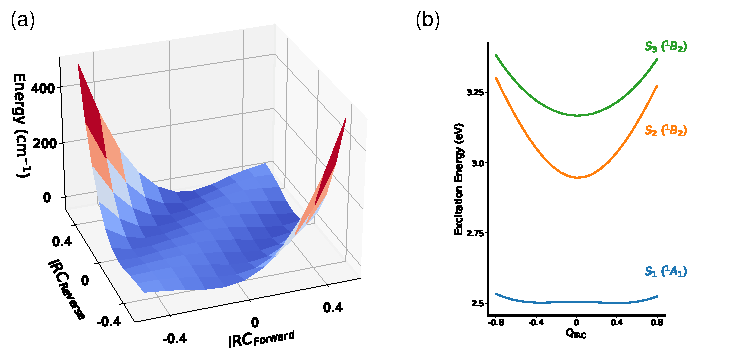
\includegraphics[width=0.8\textwidth]{figures/Figure2}
	\caption{(a) A 2D representation of the $\text{S}_1$ excited state surface of 9H-An$^+$, along the forward and reverse IRC coordinates. The surface consists of 100 grid points calculated at the M06-2X/cc-pvtz level. The surface shows the two global minima, connected by a shallow (35~cm$^{-1}$) saddle point. (b) Higher excited state potential energy curves along a single IRC coordinate. The large energy separation between the $\text{S}_1$ and $\text{S}_2$ states, combined with the double well potential, reflects a two-state avoided crossing model. This suggests the presence of a strong adiabatic interaction between the $\text{S}_1$ and $\text{S}_2$ surfaces. }
	\label{Fig:2}
\end{figure}

To visualise the charge transfer event, electrostatic potential surfaces were evaluated at both the $C_{2v}$ and $C_s$ geometries, as shown in Figure~\ref{Fig:3}. The surfaces confirm that the positive charge largely resides on the sp$^{2}$ bridge at the ground state $C_{2v}$ geometry. During excitation to the $\text{S}_1$ state, the hole hops onto one of the aromatic rings, where it remains localised at the excited $C_s$ geometry. This charge-hopping coordinate resembles a Marcus-Hush system, confirming that protonated anthracene is an excellent prototype for the study of intramolecular hole$-$transfer.

\begin{figure} [h]
	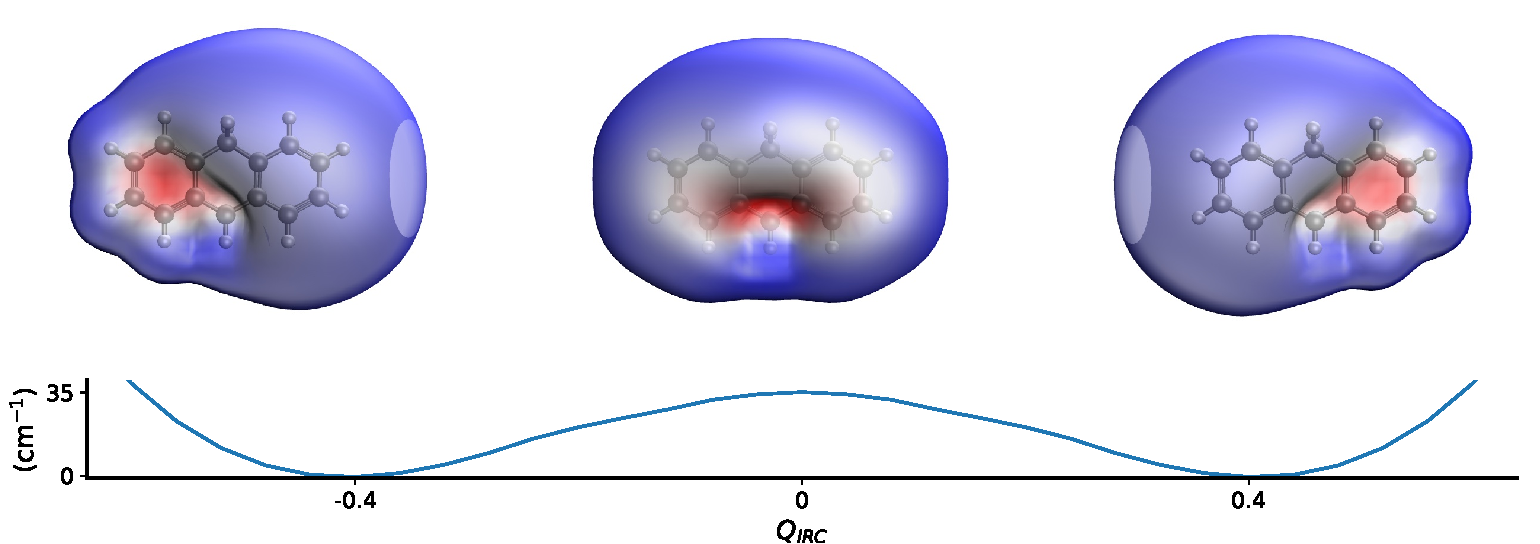
\includegraphics[width=0.8\textwidth]{figures/Figure3W}
	\caption{Calculated charge density plots of 9H-An$^+$ at the $C_{2v}$ transition state geometry reveals that the hole is largely located on the bridge. Conversely, density plots at either of the $C_s$ excited geometries show the hole remains largely localised on one of the aromatic rings. Therefore, the 9H-An$^+$ cation represents an example of photo-induced charge transfer, as excitation of the molecule will result in the hole hopping from the central bridge onto one of the terminal rings.}
	\label{Fig:3}
\end{figure}

\section{Results and Discussion}
\subsection{9H-An$^+$}
The triple resonant photodissociation spectrum of protonated anthracene is shown in Figure~\ref{Fig:4}. The cations were prepared by resonantly ionizing the neutrals at threshold, and as such we can be certain that the spectra correspond to protonation (deuteronation) at the 9-position, the $C_{2v}$ species. The spectra reveal a number of progressions, possibly indicating a large geometry change between the ground and excited states of the cation. While the lowest energy geometry for the excited state possess $C_s$ symmetry, we may treat the excited state as approximately $C_{2v}$ as the transition state barrier (35~cm$^{-1}$) is below the calculated zero point energy.  

\begin{figure} [h]
	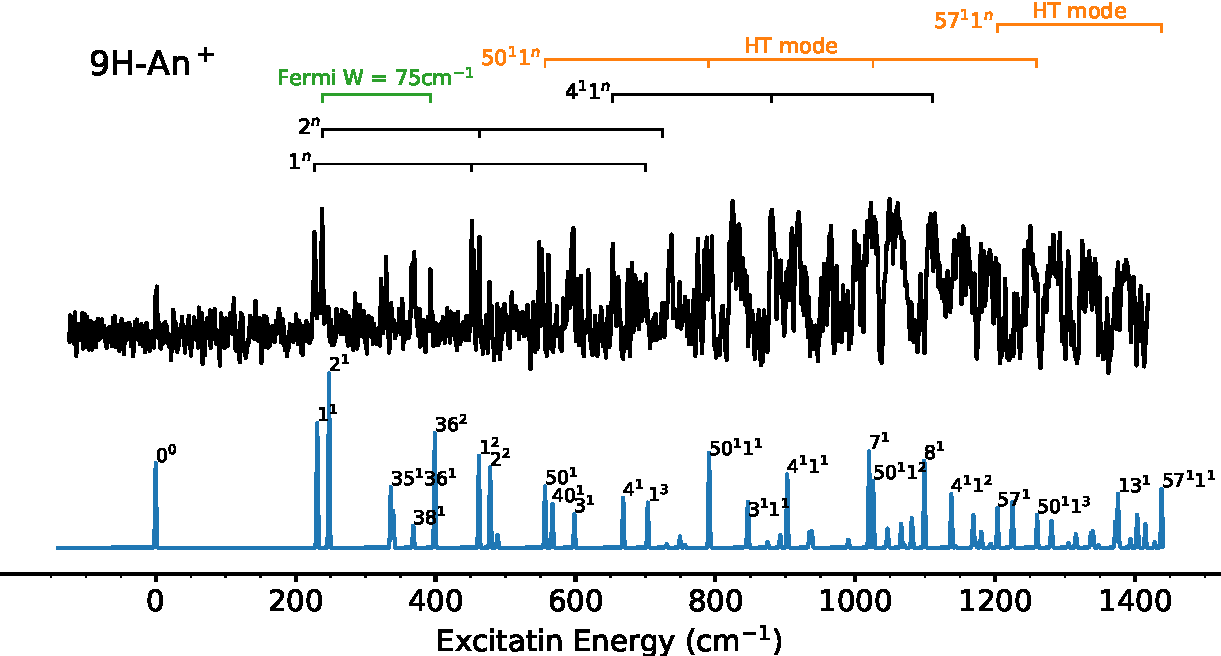
\includegraphics[width=1\textwidth]{figures/9H-An+sw}
	\caption{Triple resonance photodissociation spectrum of the S$_1$ $\leftarrow$ S$_0$  transition of 9H-An$^+$. The origin position is at 20,341~cm$^{-1}$, in agreement with the initial assignment by Alata~\emph{et al.}~\cite{ala10} The simulated spectrum, including Franck-Condon, anharmonic Fermi resonances, and Herzberg-Teller calculations at the M06-2X/cc-pvtz level, is shown for comparison in blue. The simulated spectrum closely resembles the experimental one, recreating all of the key features. The spectral structure is dominated by vibrational progressions $1^n$, $2^n$, and $4^11^n$, Herzberg-Teller coupled progressions $50^11^n$ and $57^11^n$, and a strong Fermi resonance between transitions $2^1$ and $36^2$. }
	\label{Fig:4}
\end{figure}

The $\text{S}_1\leftarrow \text{S}_0$ origin is at 20,341~cm$^{-1}$, in agreement with the previous PIMS measurement by Alata~\emph{et al.}~\cite{ala10}, confirming their assignment to the 9H-An$^+$ isomer. Multiple narrow transitions are observed up to 1,400~cm$^{-1}$ above the origin transition, that were not resolved in any of the previous studies. Spectral features below $\sim800~$cm$^{-1}$ appear sharp, with an average FWHM of $\sim 2.6~$cm$^{-1}$, while peaks at higher energies appear broader. This is likely due to the shorter dissociation lifetime of these excited vibrational states. It should also be noted that the relative intensity of peaks may be limited by saturation effects, where all of the resonant ground state cation signal is depleted.

As shown in Figure~\ref{Fig:4}, most of the structure observed in the experimental spectrum may be accounted for by a standard Franck-Condon (FC) simulation. Vibrational frequency calculations were computed at the M06-2X/cc-pvtz level for both the Ground $C_{2v}$ and excited transition state $C_{2v}$ geometries. Overlaps between the ground and excited state vibrational wavefunctions were then calculated, including Duschinsky rotations, to simulate the vibronic spectrum. The resulting spectrum was dominated by progressions in the $a_1$ symmetric $1^n$, $2^n$, and $4^11^n$ modes. Excellent agreement between the simulation and experiment was obtained for the $1^n$ and $4^11^n$ progressions, however the pure FC simulation could not account for the splitting observed near $\sim230~$cm$^{-1}$. 

To evaluate whether the splitting could be caused by a 1-2 Fermi resonance with the $1^1$ transition, anharmonic frequency analysis was performed using Generalised 2nd-order Vibrational Perturbation Theory, with 3rd and 4th derivatives also calculated at the M06-2X/cc-pvtz level~\cite{bio12}. This revealed a large Fermi resonance between modes v$_2$(366~cm$^{-1}$) and 2$\times$v$_{36}$(186~cm$^{-1}$), with a coupling strength
\begin{equation}
W = \frac{\sqrt{\Delta^2-\Delta_0^2}}{2} =75.5~\text{cm}^{-1},
\label{eq:1}
\end{equation} 
where $\Delta$ is the splitting due to the anharmonic coupling, and $\Delta_0$ is the expected transition separation without coupling~\cite{bur10}. Hence, the doublet feature at $\sim230~$cm$^{-1}$ is not from a Fermi resonance with transition $1^1$ as was expected, but instead from a large interaction between transitions $2^1$ and $36^2$. The relative intensity of the resonant peaks is given by,
\begin{equation}
\frac{I_{v2}}{I_{2\times v36}} = \frac{\left(\Delta+\Delta_0\right)}{\left(\Delta-\Delta_0\right)}=1.08.
\label{eq:2}
\end{equation}

Further features missing from the pure FC simulation may be accounted for by considering potential Herzberg-Teller vibronic coupling between the $\text{S}_1~(^1A_1)$ and $\text{S}_2~(^1B_2)$ excited states, as predicted from Figure~\ref{Fig:2}(b). Coupling would occur through b$_2$ vibrational promoter modes, as for $C_{2v}$ symmetry
\begin{equation}
^1A_1 \otimes b_2 = ^1B_2.
\label{eq:3}
\end{equation}

To account for the nuclear-electronic interactions, the Herzberg-Teller expansion may be applied to the vibronic wavefunction of the $\text{S}_1$ state $\Psi_{S_1j}(r,Q)$. By expanding around the equilibrium geometry $Q_0$, the wavefunction may be rewritten as 
\begin{equation}
|\Psi_{\text{S}_1j} \rangle = |\psi_{\text{S}_1} \chi_{\text{S}_1j} \rangle + \gamma_{\text{S}_2k,\text{S}_1j}Q_n|\psi_{\text{S}_2} \chi_{\text{S}_2k}\rangle, 
\label{eq:4}
\end{equation}
where $\psi_{\text{S}_n}$ is the electronic wavefunction of the $\text{S}_n$ state, $\chi_{\text{S}_nj}$ is the corresponding vibrational wavefunction, $Q_n$ is the coupling coordinate, and $\gamma_{\text{S}_2k,\text{S}_1j}$ is the vibronic mixing coefficient.

The strength of any vibronically coupled transitions may be determined by examining the
transition dipole moment. Substituting the $\text{S}_1$ state wavefunction from Eq.~(\ref{eq:4}) into the $\text{S}_1\leftarrow \text{S}_0$ transition dipole moment gives,
\begin{align}
\mu_{\alpha}&=\langle\Psi_{\text{S}_0}|\vec{\mu}_{\alpha}|\Psi_{\text{S}_1}\rangle\\
&=\langle\psi_{\text{S}_0}|\vec{\mu}_{\alpha}|\psi_{\text{S}_1}\rangle\langle\chi_{\text{S}_0i}|\chi_{\text{S}_1j}\rangle +
\gamma_{\text{S}_2k,\text{S}_1j}\langle\psi_{\text{S}_0}|\vec{\mu}_{\alpha}|\psi_{\text{S}_2}\rangle\langle\chi_{\text{S}_0i}|Q_n|\chi_{\text{S}_2k}\rangle\\
&=\mu_{\alpha}^{\text{S}_1-\text{S}_0}\langle\chi_{\text{S}_0i}|\chi_{\text{S}_1j}\rangle + \gamma_{\text{S}_2k,\text{S}_1j}\mu_{\alpha:0}^{\text{S}_2-\text{S}_0}\langle\chi_{\text{S}_0i}|Q_n|\chi_{\text{S}_2k}\rangle,
\label{eq:5}
\end{align}
where the term $\mu_{\alpha}^{\text{S}_1-\text{S}_0}= \langle\psi_{\text{S}_0}|\vec{\mu}_{\alpha}|\psi_{\text{S}_1}\rangle$ represents the $\text{S}_1~\leftarrow~\text{S}_0$ electronic transition moment at the ground state geometry along axis $\alpha$.

Another way to describe the vibronic coupling dependence on the transition moment would be to expand the general $\mu_{\alpha}^{\text{S}_1-\text{S}_0}$ transition dipole function as a Taylor series in $Q_n$ about the ground state geometry,
\begin{equation}
\mu_{\alpha} = \mu_{\alpha}^{\text{S}_1-\text{S}_0}\langle\chi_{\text{S}_0i}|\chi_{\text{S}_1j}\rangle + \left(\frac{\partial\mu_{\alpha}^{\text{S}_1-\text{S}_0}}{\partial Q_n}\right)_0 \langle\chi_{\text{S}_0i}|Q_n|\chi_{\text{S}_2k}\rangle + \dots 
\label{eq:6}
\end{equation} 
Comparing Eq.~(\ref{eq:5}) and Eq.~(\ref{eq:6}) one obtains,
\begin{equation}
\left(\frac{\partial\mu_{\alpha}^{\text{S}_1-\text{S}_0}}{\partial Q_n}\right)_0 = \gamma_{\text{S}_2k,\text{S}_1j}\mu_{\alpha}^{\text{S}_2-\text{S}_0}.
\label{eq:7}
\end{equation}

This shows that the strength of the possible Herzberg-Teller transitions may be estimated by calculating the derivative of the transition dipole moment along each $b_2$ normal mode coordinate. This was calculated for all 22 $b_2$ modes in protonated anthracene, along each axis, with the dipole derivatives given in the Supplementary Information. Two vibrational modes were found to have large transition dipole moment slopes, $v_{50}$ and $v_{57}$. The transition strengths of the Herzberg-Teller coupled modes can be quantified from the TD-DFT calculations by implementing a linear variation of the dipole moment to include the first order term of the Taylor expansion about the equilibrium geometry~\cite{bai13}. The resulting transition intensities were added to the simulation in Figure~\ref{Fig:4}, which included two dominant progressions $50^11^n$ and $57^11^n$. 


By combining the information from the harmonic FC, anharmonic resonances, and Herzberg-Teller calculations, the complete $\text{S}_1\leftarrow \text{S}_0$ spectrum could be simulated, as was shown in Figure~\ref{Fig:4}. The calculated spectrum resembles a close match to the experimental triple resonance photodissociation spectrum, validating the shallow double well framework and $C_{2v}$ approximation used in this work to describe the system. The majority of the spectral structure can be accounted for by a series of combination bands involving the $v_1(a_1)$ symmetric in-plane wag mode, which is possibly involved in the initial excitation from the $C_{2v}$ ground state to the $C_{2v}$ excited transition state geometry. A full list of spectral assignments is presented in the Supplementary Information.

\subsection{Charge-Transfer Coordinate}
The photo-induced charge-transfer process may be understood by considering the vibrational motion involved in the symmetry-breaking geometry change from $C_{2v}$ to $C_s$. The normal mode coordinates that point in the same direction as the intrinsic reaction coordinate can be identified by calculating the cosine similarity,
\begin{equation}
	\cos(\theta) = \frac{Q_n\cdot Q_{\text{IRC}}}{||Q_n||~||Q_{\text{IRC}}||} = \frac{1}{25} \displaystyle\sum_{j=1}^{25}\frac{q_j(x,y,z)\cdot r_j(x,y,z)}{||q_j(x,y,z)||~||r_j(x,y,z)||},
\end{equation}
where $Q_n$ is the normal mode coordinate and $Q_{\text{IRC}}$ is the intrinsic reaction coordinate from Figure~\ref{Fig:2}. Cosine similarities were calculated for each normal mode coordinate of the C$_{2v}$ excited transition state by summing over the 3-D vector overlaps for each atom in the molecule. The resulting similarities are shown for each vibrational mode in Figure~\ref{Fig:5}.

\begin{figure} [h]
	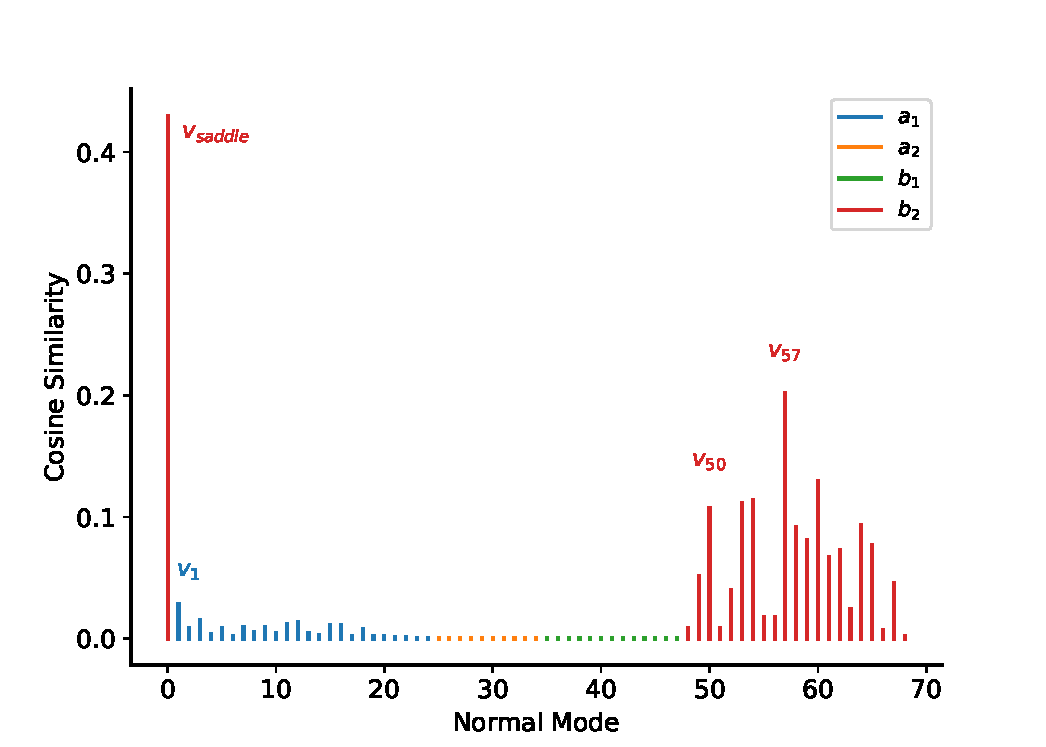
\includegraphics[width=0.5\textwidth]{figures/Figure5}
	\caption{Cosine Similarity measurements between the IRC coordinate and each normal mode of the $C_{2v}$ excited transition state of 9H-An$^+$. The normal mode coordinates were calculated at the M06-2X/cc-pvtz level. The corresponding cosine similarities were then calculated for each mode by summing the vector overlaps for each atom in the molecule. Similarities were calculated in both the forward and reverse direction, with the largest similarity for each mode shown in this figure. This highlights that the symmetry breaking coordinate is described by in-plane $b_2$ motion. Prominent modes in the triple resonance spectrum, all have relatively large Similarities, confirming that the active modes point in the same direction as the charge-transfer coordinate.}
	\label{Fig:5}
\end{figure}

Unsurprisingly, the imaginary $b_2$ saddle point frequency was the closest to the IRC coordinate. Other in-plane $b_2$ modes also point in the same direction, including modes $v_{50}$ and $v_{57}$. These Herzberg-Teller coupled modes are active in the triple resonance photodissociation spectrum in Figure~\ref{Fig:4}, confirming that they are likely involved in the hole-transfer process. %add mode description
Notably, no single mode lies predominately along the IRC, instead it must be described by a combination of different in-plane $b_2$ vibrations. Therefore, the charge-transfer process is not mediated by a single vibrational excitation.

\subsection{9D-An$^+$}
To investigate the system further, the deuterated cation 9D-An$^+$ was also studied. The cations were prepared by resonantly ionizing the 9D-dihydroanthracenyl neutral radicals at threshold, generating cold cations deuterated exclusively at the 9-position. The resulting triple-resonant photodissociation spectrum of 9D-An$^+$ is shown in Figure~\ref{Fig:6}. The experimental spectrum is shown alongside a simulated spectrum that was constructed through the combination of FC, anharmonic, and Herzberg-Teller vibronic coupling calculations, using the same method that was described for 9H-An$^+$ above.

\begin{figure} [h]
	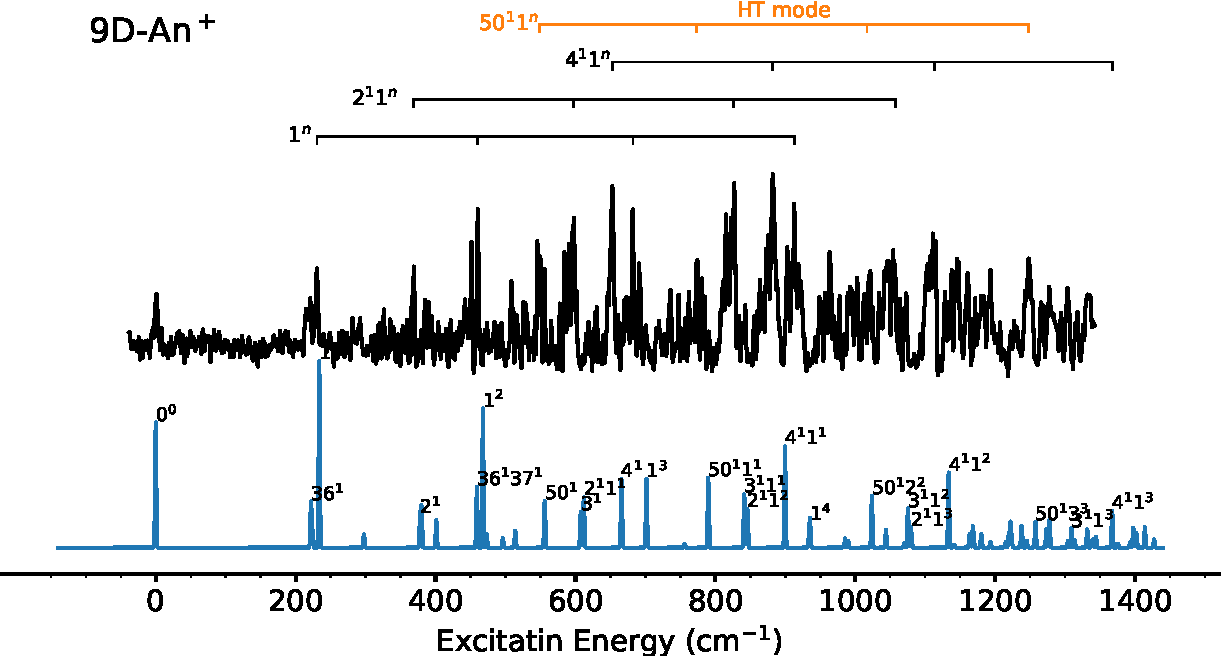
\includegraphics[width=1\textwidth]{figures/9D-An+sw}
	\caption{Triple resonance photodissociation spectrum of the S$_1$ $\leftarrow$ S$_0$  transition of 9D-An$^+$. The origin position is at 20,358~cm$^{-1}$, shifted by 17~cm$^{-1}$ from the origin position of 9H-An$^+$. The simulated spectrum, including FC, anhamronic Fermi resonances, and Herzberg-Teller calculations at the M06-2X/cc-pvtz level, is shown for comparison in blue. Again, the simulated spectrum closely resembles the experimental one, recreating all of the key features. The spectral structure is dominated by vibrational progressions $1^n$, $2^11^n$, and $4^11^n$, and the Herzberg-Teller coupled progression $50^11^n$. There is no Fermi resonance in 9D-An$^+$. }
	\label{Fig:6}
\end{figure}

Only small changes are observed between the 9H-An$^+$ (Figure~\ref{Fig:4}) and the 9D-An$^+$ (Figure~\ref{Fig:6}) spectra. In the deuterated spectrum, the origin transition is shifted by 17~cm$^{-1}$ to $20,358$~cm$^{-1}$. Again, the structure is dominated by progressions involving the $v_1 (a_1)$ symmetric in-plane wag mode, including progressions $1^n,~2^11^n,~$and$~4^11^n$. No Fermi resonance is observed in 9D-An$^+$, due to the shifts in the vibrational frequencies. A second peak is still observed near the $1^1$ transition, however it is much lower in intensity. This is assigned to the anharmonically coupled transition $36^1$. Herzberg-Teller coupled transitions are also observed, including the prominent progression $50^11^n$. A full list of spectral assignments is given in the Supplementary Information.

The effect of deuteration is much smaller than what has been observed previously for the neutral analogous dihydroanthracenyl radicals. Resonant two-colour two-photon ionisation (R2C2PI) spectra of isomer selected 9H-An and 9D-An reported previously by our group revealed a large change after deuteration, with a doubling of the number of spectral lines observed~\cite{kre19}. This was attributed to quantum-induced symmetry breaking, where the addition of a deuterium atom causes an imbalance in the zero point energy, generating an asymmetric well potential where the effective (vibrationally averaged) geometry of the excited state is bent. Therefore, the absence of a similar effect in the cation spectra of this work confirms that the 9H-An$^+$ and 9D-An$^+$ excited state geometries are both planar.

\section{Conclusions}
Triple resonance photodissociation spectra of the S$_1$ $\leftarrow$ S$_0$ excited state of 9H-An$^+$ and 9D-An$^+$ were measured, from cold cations produced in their ground vibrational state. The cations were generated resonantly from  9-dihydroanthracenyl radicals, to ensure protonation/deuteration was exclusively in the 9-position. The isomer selected spectra revealed many narrow features, not observed in previous studies. Full anharmonic and vibronic coupling calculations were able to recreate the prominent features observed in the experimental spectrum, allowing for detailed assignment of the spectral structure. Only small changes were observed in the spectra upon deuteration, supporting the notion that the S$_1$ excited stated geometries are planar.

TD-DFT calculations mapped out the S$_1$ surface, confirming that S$_0$ $\leftarrow$ S$_1$ excitation induces a charge-transfer process, where the positively charged hole hops from the sp$^2$ bridge onto one of the aromatic rings. This charge-transfer event induces a symmetry-breaking distortion, reducing the cation to C$_s$ symmetry. Signatures of this process are observed in the experimental triple resonance spectra, through the observation of Herzberg-Teller coupled $b_2$ modes $v_{50}$ and $v_{57}$. This work demonstrates how the complexities of charge-transfer processes, which are critical to the development of OPV devices, can be interrogated at a quantum-level on an individual isolated molecule.

\section{Methods}
\subsection{Experimental Details}
The experimental apparatus and triple resonance method have been described in detail in refs~\onlinecite{kre13} and~\onlinecite{kre19}. A sample of anthracene is heated to 100$^\circ$C and seeded in 5 bar of a argon/water vapour gas mixture. The water was externally heated (50$^\circ$C) and provides an excellent source of hydrogen atoms for protonation. Heavy water was used for the deuteration experiments. The seeded gas mixture is expanded into a differentially pumped source chamber, through a pulsed discharge nozzle (PDN). A discharge of 2.1~kV struck for 130~$\mu$s to generate the dihydroanthracenyl radicals. The coldest part of the beam expansion passes through a 2mm diameter skimmer, into a second differentially pumped chamber.

9H-An$^+$ and 9D-An$^+$ cations are then generated through two-colour two-photon ionisation. A fixed excitation laser at 523~nm resonantly excited the radicals to the origin band of the D$_1$ state. This confirms only radicals protonated/deuterated at the 9-position are selected. A second fixed excitation laser at 312~nm then ionises the excited radicals at threshold, ensuring cations are generated in their ground vibrational state. A third laser is then introduced, and scanned across the energy region of the cation excited state (495-457~nm). When this laser is resonant with a S$_0$ $\leftarrow$ S$_1$ vibronic transition two photons can be absorbed, with the first exciting the cation into the S$_1$ state, which then allows a second photon to dissociate the cation. This resonant dissociation results in a depletion of the overall cation signal detected. Therefore, recording this depleted signal as the third laser is scanned generates a cold, isomer selected, excitation spectrum. A Jablonski diagram explaining the experimental scheme is illustrated in Figure~\ref{Fig:7}.

\begin{figure} [h]
	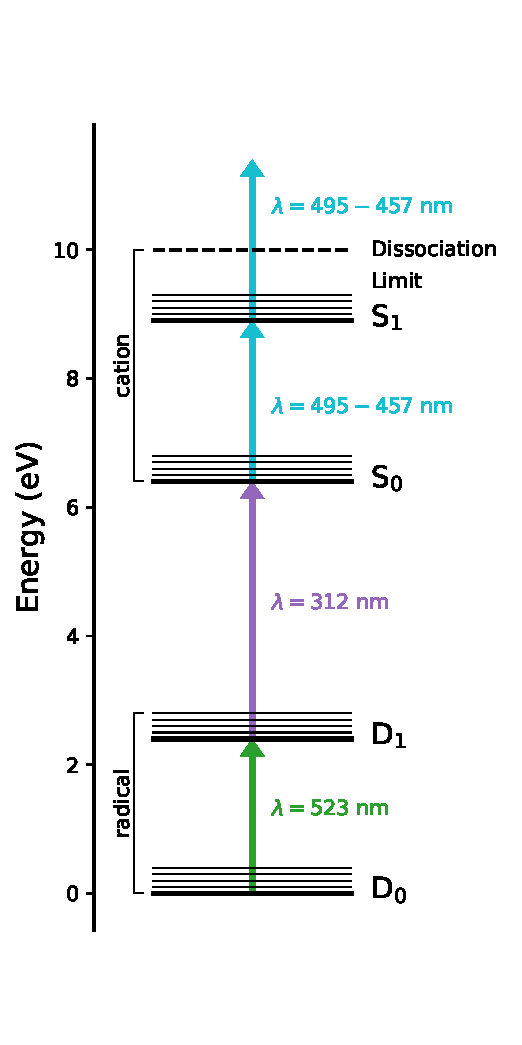
\includegraphics[width=0.3\textwidth]{figures/Figure7}
	\caption{Experimental scheme. Jet-cooled ground state dihydroanthracenyl radicals are resonantly ionised at threshold to yield isomer-selected, cold 9H-An$^+$ cations. The cation signal is depleted by resonant excitation through the S$_1$ state, followed by photodissociation. }
	\label{Fig:7}
\end{figure}

\subsection{Computational Details}
Quantum chemical computations were performed using the Gaussian-16 program~\cite{g16}. The M06-2X/cc-pvtz level of theory was utilised to perform geometry optimisations and frequency calculations of the ground and excited states. This was also used in the transition state search, and calculation of the intrinsic reaction coordinate. The planarity of the optimised geometries was confirmed by CCSD/cc-pvdz and EOM-CCSD/cc-pvdz geometry optimisations. The frequency calculations verified that all stationary points possess zero imaginary frequencies, except for the $C_{2v}$ transition state which has one. The intrinsic reaction coordinate calculations confirmed the connectivity of the transition and excited state geometries. Franck-Condon, anharmonic, and Herzberg-Teller coupling calculations involved in the spectra simulations were all carried out at the M06-2X/cc-pvtz level using Gaussian-16.

\begin{acknowledgement}
	This research was supported by the Australian Research Council Discovery
	Project Grant DP190103151.  
\end{acknowledgement}

% Create the reference section using BibTeX: 
\bibliography{AnH+}

\newpage
\onecolumn
\subsection{TOC Graphic - For Table of Contents Only}
\vspace{2ex}
\begin{center}
%	\includegraphics[width=8.5cm]{figures/TOC}
\end{center}

\end{document}
% ****** End of file apstemplate.tex ******